%Je nach dem in welcher Sprache ihr euer Paper schreiben wollt,
%benutzt bitte entweder den Deutschen-Titel oder den Englischen (einfach aus- bzw. einkommentieren mittels '%')

%Deutsch
%\section{Methodischer Ansatz}

%Englisch
\section{Methodological Approach}

\subsection{Use Case Description}
This research focuses on optimizing energy consumption for SMEs with on-premise server infrastructure
through real-time monitoring and dynamic pricing integration. The use case addresses the growing
challenge of rising energy costs that significantly impact operational expenses for small and medium
businesses. In today's volatile energy markets, SMEs face particular difficulties in understanding
and optimizing their server infrastructure's energy usage, especially in relation to fluctuating
electricity prices.

The primary objective of this use case is to create a comprehensive energy monitoring system that
collects real-time consumption data from both a smart meter and connected server equipment while
simultaneously integrating dynamic pricing information from energy markets such as EPEX Spot.
By combining these data streams, the system aims to provide SME operators with actionable insights
through intuitive dashboards that enable informed decision-making regarding server workload
scheduling and energy usage patterns.

This approach allows for the exploration of how IoT devices, cloud computing and data analytics can
be combined to create a responsive energy management solution specifically tailored for SME server
environments. The use case examines how businesses can benefit from having access to both their
server consumption patterns and market conditions in a unified interface. By making this
information accessible and understandable, SMEs can potentially shift energy-intensive computational
tasks to periods of lower pricing, resulting in cost savings without compromising operational
requirements.

\subsection{Prototype}
The prototype implements a serverless cloud architecture on Amazon Web Services (AWS) to collect,
process, and visualize energy data from multiple sources. Figure 1 illustrates the system
architecture and data flow of our solution.

\begin{figure}[htbp]
    \centering
    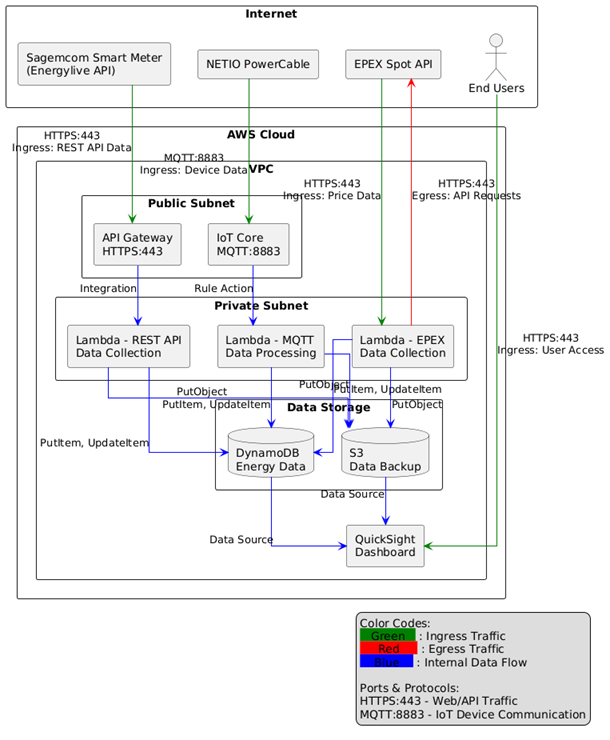
\includegraphics[width=0.6\textwidth]{fig/architecture2.png}
    \caption{System Architecture of the AWS implementation}
    \label{fig:architecture}
\end{figure}

The prototype consists of three main components that work together to deliver a comprehensive
energy monitoring solution for SME server environments. The data collection layer interfaces with
external devices and services to gather the necessary information. The Sagemcom Smart Meter
connects to the system via the Energylive API, providing facility-level energy consumption data at
ten second intervals. This data includes overall electricity usage for the entire server room or IT
infrastructure. The NETIO PowerCable device serves as an IoT sensor that measures power consumption
of individual servers and critical IT equipment, offering granular insights into which systems
contribute most significantly to the overall energy footprint. Additionally, the system integrates
with the EPEX Spot API to retrieve real-time and forecasted electricity market prices, which
are essential for cost optimization strategies.

The processing layer leverages AWS Lambda functions to handle the incoming data streams
efficiently. An API Gateway serves as the entry point for REST API requests from the smart meter,
ensuring secure and scalable communication. IoT Core manages MQTT connections from the NETIO
PowerCable device, providing a reliable communication channel for this IoT sensor.
Three specialized Lambda functions handle different aspects of data processing: one dedicated to
REST API data collection from the smart meter, another processing MQTT messages from the IoT device
and a third specifically handling EPEX market data. This separation of concerns allows for
independent scaling and maintenance of each data processing pipeline while minimizing operational
overhead for SMEs with limited IT resources.

The storage and visualization layer ensures that data is both persistently stored and meaningfully
presented to SME operators. DynamoDB serves as the primary database, storing structured energy
consumption and pricing data in a format optimized for quick retrieval and analysis. S3 provides
backup storage and handles larger datasets that might be needed for long-term trend analysis. The
QuickSight service delivers interactive dashboards to end users, allowing them to explore their
server energy usage patterns, correlate consumption with pricing data, and identify optimization
opportunities through intuitive visualizations and reports that don't require specialized data
science expertise.

The architecture follows security best practices by implementing a Virtual Private Cloud (VPC) with
public and private subnets. External communications occur through secure protocols
(HTTPS for API traffic and MQTT over TLS for IoT devices), while internal data flows are restricted
within the VPC. This design ensures that sensitive consumption data remains protected while still
allowing for the necessary external integrations, addressing the security concerns that are
particularly important for SMEs handling sensitive business data.

\subsection{Measurement}
To evaluate the effectiveness of our approach, we will implement a comprehensive measurement
framework that addresses technical performance, server energy consumption patterns, and economic
impacts. This multi-faceted evaluation will provide insights into both the system's technical
capabilities and its practical utility for SME operators.

From a system performance perspective, we will measure several key technical metrics to ensure the
solution meets the necessary requirements for a production environment in an SME context. Data
collection latency will be carefully monitored to determine the time between actual energy
consumption events and the availability of this data within the system. This metric is crucial for
near real-time applications, particularly when operators might make decisions about server workload
scheduling based on current consumption patterns and electricity prices. We will also assess
processing throughput by measuring the number of data points the system can handle per minute,
ensuring it can scale to accommodate multiple servers and frequent reporting intervals without
requiring expensive infrastructure. System reliability will be evaluated through comprehensive
monitoring of uptime percentages and error rates across all components, with particular attention
to the critical data collection pathways.

Server energy consumption analysis forms the core of our measurement approach. We will track total
energy usage in kilowatt-hours across various time periods (hourly, daily, weekly, and monthly)
to establish baseline consumption patterns and identify trends in server utilization. Detailed
temporal analysis will reveal usage patterns throughout the day, highlighting peak usage times
and baseline consumption levels that might represent always-on services or idle power states.
The device-specific consumption data from the NETIO PowerCable devices will allow for granular
analysis of which servers or systems contribute most significantly to overall energy usage,
providing targeted opportunities for optimization. We will also correlate energy consumption with
specific workloads and server utilization metrics to develop energy profiles for different
operational scenarios.

The economic dimension of our measurement framework will focus on establishing the financial impact
of the system for SMEs. We will analyze cost correlation by examining the relationship between
energy prices from the EPEX Spot market and server consumption patterns, determining whether
workloads naturally align with lower-price periods or if intervention is needed. Potential savings
will be calculated by modeling the difference between current usage patterns and theoretically
optimized scenarios where energy-intensive computational tasks are shifted to lower-price periods.
A comprehensive return on investment analysis will evaluate the cost-benefit relationship of
implementing the system versus the potential savings achieved through optimized energy usage, with
specific attention to the financial constraints and considerations typical of SMEs.

The collected data will undergo rigorous statistical analysis to identify patterns and correlations
between server energy consumption, market prices, and external factors such as time of day, day of
week, and seasonal variations. Machine learning techniques may be applied to detect anomalies in
consumption patterns and predict future usage based on historical data. This analytical approach
will provide insights into potential optimization strategies and validate the effectiveness of the
proposed solution in achieving its goals of reducing energy costs for SMEs while maintaining
operational performance and reliability of their server infrastructure.

Through this comprehensive measurement framework, we aim to demonstrate not only the technical
feasibility of our approach but also its practical utility in helping SMEs make informed decisions
about their server energy consumption in relation to dynamic market conditions, ultimately
contributing to both cost savings and environmental sustainability.

